

\documentclass[chapter, oneside]{oblivoir}
\usepackage{kotex}

% 뭐임
\usepackage{amsmath}
\usepackage{amssymb}
\usepackage{amsthm}
\usepackage{graphicx}
\usepackage{mathtools}




%--------- 멋대로 정의해본 명령어
\newcommand{\dx}[1]{\operatorname{d}\! #1}
\newcommand{\term}[1]{\textbf{#1}}




\title{푸리의 변환의 수학적 원리}
\author{esctabcapslock }


\begin{document}
\maketitle



이 상태로 보고서를 마무리하기에는, 푸리에 변환 자체를 수학적으로 접근하지 않은 것과, 내가 사용한 알고리즘에 대해 잘 모른다는 사실이 마음에 걸렸음.
따라서, 위의 탐구를 다 마친 뒤, 푸리에 변환에 관한 수학 이론적인 조사를 추가로 진행함.

※ https://blog.myungwoo.kr/54의 자료를 나름대로 이해, 본인 수준의 언어로 정리한 것임.


\section{변환이 성립하는 직관적 이유 }
푸리에 변환의 입출력 데이터를 각각 $\vec{N}$차원의 백터로 생각하자.
각 백터 $\vec{a}$의 $k$번째 성분을 $\vec{a}(k)$라고 표기하겠다.
그리고 두 차원 복소 백터의 내적을 다음과 같이 정의하자
$${\vec{a}} \cdot  {\vec{b}} = \sum _{n=0} ^{N-1} \vec{a}(n) \overline{ \vec{b}(n)} \quad \text{(}\bar{b}\text{는 }b\text{의 컬례 복소수)}$$
그리고 ${\vec{\phi  _{k}}}$를 다음과 같이 정의하자.
$$ \vec{\phi_k}(n) = exp \left( {2 \pi k} \over {N} n \right) =w _{N}^{kn} \quad (w _{N}\text{은 1의 }N\text{제곱근)}$$
그려면, 임의의 정수 $k$, $l$ (단,$k \neq l$ )에 대해서,$\vec{\phi  _{k}} \cdot  \vec{\phi_l} = \vec{0}$  성립. $\cdots$ⓐ 
\footnote{위 정의에 대입한 뒤, 등비급수 공식을 적용해 전개해 보면 분자가 0이 됨}





즉, $\vec{\phi_0}$, $\vec{\phi_1}$, $\cdots$,  $\vec{\phi_{N-1}}$은 서로 직교하는 백터로, $N$차원 공간의 일차독립인 기저들이라고 생각할 수 있다.

푸리에 변환의 입력 데이터가 $\vec{a}$, 출력 결과가 $\vec{A}$라면, 푸리에 변환은 다음과 같이 표현할 수 있다.
$$\vec{A}(n)= \vec{a} \cdot \vec{\overline{\phi_n}}$$
즉, 푸리에 변환이란 기존의 백터 $\vec{a}$를, 새로운 기저 $\vec{\phi_0}$, $\vec{\phi_1}$, $\cdots$,  $\vec{\phi_{N-1}}$들을 활용해 새롭게 표현한 것이라고 이해할 수 있다.


\section{푸리에 역변환 증명}
$$\vec{A} \cdot \vec{\phi_1}= \sum _{n=0}^{N-1}  \vec{A}(n) \overline{\phi_l}(n) 
=\sum_{n=0}^{N-1} \left( \vec{a} \cdot  \vec{\overline{\phi_n}} \right) \overline{\phi_l(n)} $$$$
= \sum _{n=0}^{N-1}  \left( \sum_{k=1} ^{N-1} \vec{a}(k) \vec{\phi_n}(k) \right) \overline{\phi  _l}(n)$$
$$= \sum _{n=0} ^{N-1} \sum _{k=1} ^{N-1} \vec{a} (k) \overline{\vec{\phi_n}} (k) \overline{\phi_l}(n) $$

$$
= \sum _{k=1} ^{N-1}  \sum _{n=0} ^{N-1} \vec{a} (k) \vec{\phi_n}(k) \overline{\phi_l}(n) 
$$

$$= \sum _{k=1} ^{N-1} \vec{a} (k) \left( \sum _{n=0} ^{N-1} \vec{\phi_n}(k) \overline{\phi_l} (n) \right)$$

$$ =N \vec{a} (l)\footnote{
$k \neq l$이면, 괄호 한 시그마 식이 $0$이 되고,  $k = l$일 때는 $N$이 된다. ($\because$ ⓐ)}$$

즉, 이 성립한다. (역변환)


\section{고속 푸리에 변환 증명}
기함수와 우함수의 관계를 이용한다.



$N$이 $2$의 거듭제골 꼴일 때 생각하자.
푸리에 변환을 간단하게 $F$로 나타낼 것이다. $F( {\vec{a}} )= {\vec{A}}$이렇게.


$n<N/2$인 경우를 생각하자. 
$\overrightarrow{a _{\text{even}}} (n)= \overrightarrow{a} (2n)$, $\overrightarrow{a _{odd}} (n)= \overrightarrow{a_{odd}} (2n+1)$로 정의하자.

$$F( {\vec{a}} )(n)$$
$$= {\vec{a}} \cdot  {\vec{{\overline{\phi  _{n}}}}}$$
$$ = \sum _{k=0} ^{N-1} {\vec{a}} (k)w _N^{kn}$$
$$ = \sum _{k=0} ^{N/2-1} {\vec{a}} (2k)w _N^{2kn} + \sum _{k=0} ^{N/2-1} {\vec{a}} (2k+1)w _N^{(2k+1)n}$$
$$\sum _{k=0} ^{N/2-1} \vec{a} (2k)w _N^{2kn} +w _N^n \sum _{k=0} ^{N/2-1} \vec{a} (2k+1)w _N^{2kn} $$
$$=F( {\overrightarrow{a _{even}}} )(n)+w _N^n F( {\overrightarrow{a _{odd}}} )(n)$$
이다.
$n \ge N/2$인 경우, $\overrightarrow{A _{even}}$과, $\overrightarrow{A _{odd}}$의 주기가 $N/2$니까 거의 비슷한 꼴로 적을 수 있다. `'거의 비슷한''의 이유는, $w _{N}^{n}$의 부호가 바뀌는 것을 고려해야 하기 때문이다.


따라서, 기존의, 길이가 이였던 것을 짜리 2개로, 일종의 점화식 형태로 표현할 수 있다. 이것이 바로 고속 푸리에 변환(FFT)의 원리이다.

\begin{figure}[ht]
    \centering
    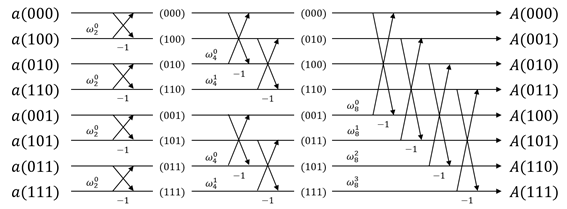
\includegraphics[width=.7\textwidth]{images/image01.png}
    \caption{콜리-튜키 알고리즘의 원리, https://casterian.net/archives/297 참조}
    \label{fig:my_label}
\end{figure}


다시 이 점화식을 컴퓨터가 계산하기 쉽도록 반복문 형태로 적절히 변형한 것이, 콜리-튜키 알고리즘, 혹은 버터플라이 알고리즘으로, 앞에서 필자가 뭣도 모르고 인터넷에서 긁어와 사용한 코드이다.



\end{document}